\section{Extension: Cultural variations in polite speech understanding}
\label{sec:culture}

US adults show understanding of polite speech as reflecting epistemic-social tradeoffs, and pilot data suggest that children in the US also show pattern consistent with the tradeoff hypothesis, especially with increasing age. Pending completion of proposed work described above, I plan to start to examine other populations of interest: different cultural groups. Based on our current model, variability might arise because different cultures may: (1) have varied literal semantic meanings of utterances; (2) place different prior expectations for a lay speaker's goals; and/or (3) place different emphases on one of these two communicative goals -- e.g. some cultures may consider it noble to try to make others feel good by lying, whereas some may regard honesty as the most important virtue. I plan to test these possibilities in the experiments described below. 

\subsection{Background} 

To the best of my knowledge, there has been no study looking at cross-cultural variations in adults' polite speech understanding. There have been only a few studies that have looked at cultural variations in children's ratings of white lies (e.g. \citealt{fu2007, ma2011}). For example, Chinese children as young as 7 years rate lie-telling as positive in a public than private situation, and as negative when accurate information would help the listener \citep{ma2011}. But these studies do not offer comparisons with European American children (cf. \citealt{lee1997}). In my proposed work, we hope to directly compare three groups of interest: US and India, and South Korea. These areas cover a wide range of languages used, religions and socioeconomic statuses, and thus will help provide a comprehensive view over the general trend of pragmatic language understanding across different cultures.

\subsection{Empirical tests}

\subsubsection{Experiment 4: Indian and Korean adults' true state inference} 
This experiment will be identical in structure as Experiment P1, and participants will reason about the true state given speaker's utterance and goal. Indian participants will be recruited on Amazon's Mechanical Turk, and Korean participants by advertising on Facebook and community websites. In order to test for linguistic (rather than cultural) differences, we will recruit participants in two batches for each site: one batch that speaks Hindi and the other that speaks English from India; and one batch for Korean and one for English from Korea, and we will compare the data to examine any differences that may arise from language.  

\subsubsection{Experiment 5: Indian and Korean adults' goal inference} 
This experiment will be identical in structure as Experiment P2, and they will reason about the true state given speaker's utterance and goal. Participants will be recruited in an identical manner to Experiment 4. 

\subsubsection{Experiment 6: US, Indian and Korean adults' social desirability judgments} The first part of this experiment will replicate Experiment P2 and 5 by asking for adult participants' goal inference given speaker's utterance and true state provided in the scenario. The second part will address the same scenario, but ask for participants' judgments for social evaluation of the speaker: (1) How likely are you [the participant] to like the speaker? (2) How likely are you to ask the speaker for feedback for your own performance? These measures of social approval will help approximate the perceived ``optimality'' of a given set of inferred goal weights; for example, participants may infer that Alice wanted to nice but not honest when she said ?it was good? about a mediocre presentation (e.g. deserving two out of five hearts), and then indicate that they are likely to like Alice, but not ask her for feedback. Participants will be recruited in an identical manner to Experiment P2 and 5.

\subsubsection{Experiment 7: Indian children's understanding of polite speech} 
This experiment will be identical in structure as Experiment 1. Participants will be recruited at elementary schools in India. The Indian site has been used extensively by PI Frank in unrelated research on mathematics \citep{frankbarner2012, barner2016}. We will recruit two different age groups (5-6 and 7-8-year-olds) matching those for Experiment 4, with a minimum of 10 and maximum of 24 participants per condition and age group, allowed by the total testing time at the field site. They will be tested in English or their native language (Hindi or Gujarati), with a script that is directly translated from English by an educated native speaker. Those who are not exposed to the language of instruction at least 75\% daily will be excluded from data analysis. 

\subsection{Results from pilot work} 

Figure~\ref{fig:expt5} shows an example analysis conducted on pilot data for Experiment 7. Whereas US children attributed more niceness to polite speaker than honest speaker with increasing age, Indian children showed the opposite trend of attributing more niceness to honest than polite speaker across both age groups. This is preliminary yet promising evidence that construal of niceness (linked to the notion of optimal tradeoff of truthfulness versus face-saving) may be different across cultures. We will seek to verify this trend with larger sample sizes to account for variability and ensure robustness of judgment patterns.

\begin{figure*}[t]
\begin{centering}
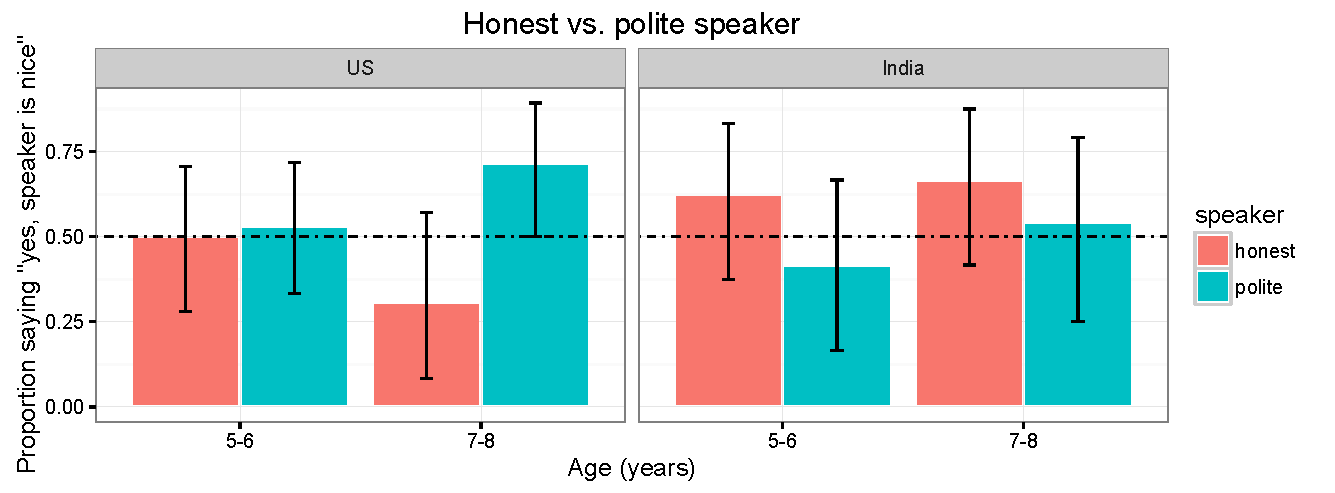
\includegraphics[width=\textwidth]{figures/exp4.pdf}
\caption{\label{fig:expt5} Results from Experiment 7 (pilot), for US versus Indian children's niceness judgments for honest versus polite (but dishonest) speaker. Error bars represent 95\% confidence intervals.}
\end{centering}
\end{figure*}

\subsection{Implications for the model}

Preliminary data from Indian child participants show an interesting reversal in speaker niceness attribution: Indian children tend to say that an honest speaker is nicer than a polite speaker. In light of our model, two interpretations are possible (if the patterns hold up): either Indian children do not reason about polite language based on epistemic-social tradeoff as we hypothesized, or Indian children have a different construal of the word ``nice,'' to mean ``helpful for future performance'' (i.e. giving useful feedback) rather than ``kind'' or ``caring''. If the latter is true, then it informs that language of instruction is a critical consideration in conducting these studies, and that Indians may have a different sense of what comprises most helpful communication from the US population. Our proposed work addresses both of these issues, in that we will conduct each Experiment at each site in two languages: the local language and English, to look at any differences in responses that are caused by language rather than cultural differences; and we will inquire what each cultural group thinks of as an optimal, cooperative speaker.


%%% Local Variables: 
%%% mode: latex
%%% TeX-master: "desc"
%%% End

